% Fig 3.4 — mDPR encoding flow
\documentclass[border=4pt]{standalone}
\usepackage{tikz}
\usetikzlibrary{positioning, arrows.meta, shapes.geometric}
\begin{document}
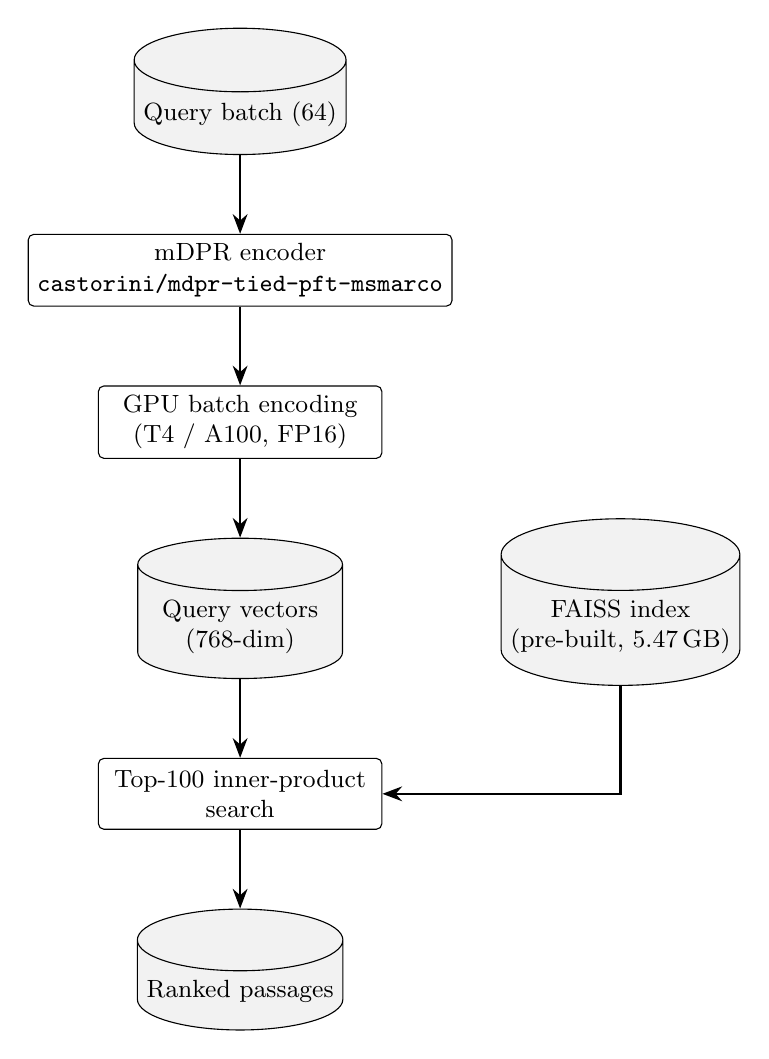
\begin{tikzpicture}[
    >=Stealth, node distance=10mm,
    box/.style={rectangle, draw, rounded corners=2pt,
                minimum width=36mm, minimum height=9mm, align=center, font=\small},
    data/.style={cylinder, shape border rotate=90, aspect=0.3, draw,
                 minimum width=26mm, minimum height=10mm, align=center,
                 font=\small, fill=black!5},
    arrow/.style={-{Stealth[length=2.5mm]}, thick}
]
  \node[data] (q) {Query batch (64)};
  \node[box, below=of q] (enc) {mDPR encoder\\\texttt{castorini/mdpr-tied-pft-msmarco}};
  \node[box, below=of enc] (gpu) {GPU batch encoding\\(T4 / A100, FP16)};
  \node[data, below=of gpu] (vec) {Query vectors\\($768$-dim)};
  \node[data, right=of vec, xshift=10mm] (idx) {FAISS index\\(pre-built, 5.47\,GB)};
  \node[box, below=of vec] (search) {Top-100 inner-product\\search};
  \node[data, below=of search] (out) {Ranked passages};

  \draw[arrow] (q) -- (enc);
  \draw[arrow] (enc) -- (gpu);
  \draw[arrow] (gpu) -- (vec);
  \draw[arrow] (vec) -- (search);
  \draw[arrow] (idx) |- (search);
  \draw[arrow] (search) -- (out);
\end{tikzpicture}
\end{document}
